\documentclass[11pt,letterpaper]{article}
\usepackage[T1]{fontenc}
\usepackage[utf8]{inputenc}
\usepackage{amsmath,amsthm,mathtools}
\usepackage{newtxtext,newtxmath}
\usepackage[margin=1in,headheight=14pt]{geometry}
\usepackage{microtype}
\usepackage{graphicx,booktabs,tabularx,array}
\usepackage{enumitem}
\usepackage{fancyhdr}
\usepackage{xurl}
\usepackage[hidelinks]{hyperref}
\usepackage{listings}
\usepackage{caption}
\captionsetup{font=small,labelfont=bf}
\setlength{\parskip}{0.3em}
\setlength{\parindent}{1.2em}
\setlength{\emergencystretch}{2em}
\linespread{1.04}
\pagestyle{fancy}
\fancyhf{}
\fancyhead[L]{\small Nonreal roots in polynomial iterative equations}
\fancyhead[R]{\small\thepage}
\renewcommand{\headrulewidth}{0.3pt}
\newtheorem{theorem}{Theorem}[section]
\newtheorem{lemma}[theorem]{Lemma}
\newtheorem{proposition}[theorem]{Proposition}
\newtheorem{corollary}[theorem]{Corollary}
\theoremstyle{definition}
\newtheorem{definition}[theorem]{Definition}
\newtheorem{example}[theorem]{Example}
\theoremstyle{remark}
\newtheorem{remark}[theorem]{Remark}
\newcommand{\R}{\mathbb R}
\newcommand{\C}{\mathbb C}
\newcommand{\Z}{\mathbb Z}
\newcommand{\N}{\mathbb N}
\newcommand{\id}{\operatorname{id}}
\newcommand{\itn}[2]{#1^{\circ #2}}
\newcommand{\Ann}{\operatorname{Ann}}
\DeclareMathOperator{\lcm}{lcm}
\DeclareMathOperator{\sgn}{sgn}
\newcommand{\abs}[1]{\left|#1\right|}
\newcommand{\norm}[1]{\left\|#1\right\|}
\newcommand{\degree}{\operatorname{deg}}
\lstset{basicstyle=\small\ttfamily,breaklines=true,columns=fullflexible,
  keepspaces=true,showstringspaces=false,frame=single,framerule=0.3pt}
\hypersetup{pdftitle={Nonreal Roots Survive in Polynomial Iterative Equations},
 pdfauthor={Research draft prepared for Vladimir Reshetnikov},
 pdfsubject={A counterexample to a published root-elimination question and a circular-spectrum classification}}
\title{\textbf{Nonreal Roots Survive\\in Polynomial Iterative Equations}\\[0.5em]
  \large A cubic counterexample and a classification of circular spectra}
\author{Research draft prepared for Vladimir Reshetnikov}
\date{20 September 2026}

\begin{document}
\maketitle
\begin{abstract}
For a real polynomial $P(z)=\sum_{j=0}^d a_jz^j$, write
$P[f](x)=\sum_{j=0}^d a_j\itn{f}{j}(x)$, where $\itn{f}{0}(x)=x$.
A published question of Draga and Morawiec asks whether nonreal characteristic
roots of maximal modulus can be removed when a real root has the same modulus.
We give a negative answer under the stated continuity assumptions. An explicit,
odd, increasing, globally bi-Lipschitz homeomorphism $F$ satisfies
$\itn{F}{3}(x)=8x$, although $F(1)=3$. Its minimal iterative polynomial is
$z^3-8$, certified by a $3\times3$ Hankel determinant equal to $-56$.
A second construction is real analytic at every real point and has minimal
polynomial $(z-1)^2(z^2+1)$; deleting its nonreal roots also fails.

We then determine exactly which monic real polynomials supported on one circle
$|z|=r>0$ occur as minimal iterative polynomials of increasing homeomorphisms of
$\R$. For $r\ne1$, the positive root $r$ must have odd multiplicity, at least
as large as every other multiplicity. For $r=1$, the identity is exceptional;
otherwise the multiplicity of $1$ must be even and strictly larger than every
other multiplicity. Every permitted polynomial is realized by an explicit
small trigonometric perturbation of a polynomial--exponential coordinate.
The proof uses two-sided orbit recurrences and an elementary positivity lemma.
We also obtain sharp increasing-solution rigidity criteria and explain the
role of differentiability at a fixed point. Exact rational verification code,
certificates, and the random area-selection record accompany the article.
\end{abstract}

\noindent\textbf{Status.} The counterexamples and classification are proved below.
This is an AI-assisted, unrefereed research draft, not a proof-assistant-checked
publication. A targeted literature search located the published open question
but did not establish priority for the answer or for the classification.
The conjugacy mechanism itself is not claimed to be new.

\clearpage
\begingroup
\small
\setlength{\parskip}{0pt}
\tableofcontents
\endgroup
\clearpage

\section{The problem selected and the scope of the answer}
\label{sec:problem}

\subsection{A precise published target}

Let $I\subseteq\R$ be a nondegenerate interval and let
$f:I\to I$ be continuous. An equation
\begin{equation}
  a_d\itn{f}{d}(x)+a_{d-1}\itn{f}{d-1}(x)+\cdots+a_1f(x)+a_0x=0
  \label{eq:iterative}
\end{equation}
with $a_0a_d\ne0$ is a polynomial-like iterative equation. Its
\emph{characteristic polynomial} is $P(z)=\sum_{j=0}^d a_jz^j$.
The notation concerns composition, not pointwise powers: in general,
$\itn{f}{2}(x)$ is not $f(x)^2$.

The specific target is Problem~6.1 of Draga and Morawiec
\cite{DM2016}, in the last section of their paper. In the context of
lowering the order of \eqref{eq:iterative}, they ask about deleting nonreal
roots of largest modulus when a real root has that same modulus. The
question also appears in the authors' preprint, page~13. Here
\emph{deleting roots} means replacing $P$ by the corresponding polynomial
divisor while preserving the implication that every solution satisfies the
lower-order equation.

The answer under these hypotheses alone is negative. In fact, the cubic
counterexample in Section~\ref{sec:cubic} satisfies no nonzero equation of
lower order whatsoever. The analytic counterexample in
Section~\ref{sec:analytic} shows that lack of smoothness is not the general
reason for failure.

The equal-modulus qualification is essential. Existing order-reduction
results employ strict separation of root moduli, together with orbit
monotonicity or alternating monotonicity; Draga's later note discusses
additional elimination cases and again identifies the unrestricted
nonreal-root issue as unresolved \cite{D2016}. Our examples do not
contradict those theorems: they lie at the spectral boundary excluded by
strict separation.

\subsection{Relation to the initial candidate}

The literature search began with Petrov's MathOverflow question asking for
conditions on $P$ that force a continuous solution of $P[f]=0$ to be linear
\cite{Petrov2016}. The retrieved question had no posted answer. It led to
the more sharply formulated root-elimination problem above.

Throughout this article, \emph{homogeneous linear} means $f(x)=cx$ and
\emph{affine} means $f(x)=cx+b$. The distinction matters when $1$ is a
multiple root. We do not claim a complete answer to Petrov's question for
arbitrary polynomials or for both monotonicity orientations. We do obtain
an exact answer for \emph{increasing solutions when all characteristic
roots lie on one circle}; see Section~\ref{sec:rigidity}.

\subsection{Random selection, exclusion, and priority}

Before choosing a problem, a list of 80 mathematical areas was supplied to
an operating-system-backed random generator through
\texttt{secrets.randbelow(80)}. The first draw returned the zero-based index
$17$: area~18, \emph{Functional equations}. There was no redraw. The complete
ordered list and the result are preserved in
\texttt{data/selection.json}.

The supplied \texttt{manifest(1).tex} was reviewed in full. The present
problem was not selected from its entries. Its SHA-256 fingerprint is
recorded with the selection so that the exclusion check can be tied to the
actual supplied version; see Appendix~\ref{app:reproduce}.

The target is therefore an explicitly published open question, not a new
question invented for this report. The search found the original statement,
subsequent related papers, and no explicit later answer. That is not an
exhaustive bibliographic certification that the question remained open up
to the preparation date. The mathematical conclusion below is independent
of that priority issue: the proposed general elimination is false as
printed. Nor should the elementary conjugacy construction be advertised as
a new technique. The contribution developed here is the explicit
counterexample, its connection with the published question, and the
self-contained spectral classification.

\section{An exact cubic counterexample}
\label{sec:cubic}

\subsection{The two-branch definition}

Define a function on one fundamental interval by
\begin{equation}
  \phi(u)=
  \begin{cases}
    (u+5)/2,&1\le u\le3,\\
    4u-8,&3\le u\le8.
  \end{cases}
  \label{eq:phi}
\end{equation}
The formulas agree at $u=3$. For $x>0$, choose the unique $k\in\Z$ such that
$8^k\le x<8^{k+1}$, and put
\begin{equation}
  F(x)=8^k\phi(8^{-k}x).
  \label{eq:Fpos}
\end{equation}
Complete the definition by
\begin{equation}
  F(0)=0,\qquad F(-x)=-F(x)\quad(x>0).
  \label{eq:Fodd}
\end{equation}
The endpoint identity $\phi(8)=24=8\phi(1)$ makes the scaling construction
consistent. It gives, on the whole real line,
\begin{equation}
  F(8x)=8F(x).
  \label{eq:scale}
\end{equation}

\begin{theorem}[Cubic counterexample]
\label{thm:cubic}
The function $F$ defined by \eqref{eq:phi}--\eqref{eq:Fodd} is an odd,
strictly increasing homeomorphism of $\R$ with
\begin{equation}
  \frac12|x-y|\le |F(x)-F(y)|\le4|x-y|\qquad(x,y\in\R).
  \label{eq:LipF}
\end{equation}
It satisfies
\begin{equation}
  \itn{F}{3}(x)=8x\qquad(x\in\R),
  \label{eq:Fcube}
\end{equation}
but is not homogeneous linear or affine. The smallest degree of a nonzero
polynomial $Q$ with $Q[F]=0$ is three, and the monic polynomial of that
degree is
\begin{equation}
  \mu_F(z)=z^3-8=(z-2)(z^2+2z+4).
  \label{eq:minF}
\end{equation}
\end{theorem}

\begin{proof}
On every scaled copy of the two intervals in \eqref{eq:phi}, the slope of
$F$ is either $1/2$ or $4$. The pieces meet continuously. Moreover,
\begin{equation}
  \frac43\le\frac{F(x)}x\le3\qquad(x>0).
  \label{eq:ratioF}
\end{equation}
For the first branch this follows from
$\phi(u)/u=1/2+5/(2u)$; for the second it follows from
$\phi(u)/u=4-8/u$. Thus $F(x)\to0$ as $x\to0$, and $F(x)\to\infty$ as
$x\to\infty$. Oddness handles the negative half-line. Strict monotonicity
and surjectivity follow.

Between two strictly positive points there are only finitely many
breakpoints, so their secant slope lies between $1/2$ and $4$.
Pass to a limit when one endpoint is zero, and use oddness and addition
across zero to obtain \eqref{eq:LipF} for all pairs of points.

To check the iterate relation it suffices to work on $[1,8]$.
There are three relevant itinerary intervals, because an intermediate
iterate crosses a breakpoint at $x=4$. Direct substitution gives
Table~\ref{tab:itinerary}. In using the table, values in $[8,64]$ are
computed with \eqref{eq:scale}. The final column is $8x$ in every row.
Scaling extends the identity to every positive $x$; oddness and the value
at zero finish the proof of \eqref{eq:Fcube}.

The values $F(1)=3$ and $F(3)=4$ show that $F$ is not homogeneous linear.
Since $F(0)=0$, it is not affine either. Minimality is proved immediately
below.
\end{proof}

\begin{table}[htbp]
\centering
\caption{Exact branchwise verification of the cubic relation.}
\label{tab:itinerary}
\begin{tabular}{llll}
\toprule
Initial interval & $F(x)$ & $\itn{F}{2}(x)$ & $\itn{F}{3}(x)$\\
\midrule
$[1,3]$ & $(x+5)/2$ & $2x+2$ & $8x$\\
$[3,4]$ & $4x-8$ & $16x-40$ & $8x$\\
$[4,8]$ & $4x-8$ & $2x+16$ & $8x$\\
\bottomrule
\end{tabular}
\end{table}

\subsection{A small exact certificate of minimality}

The orbit beginning at $1$ is
\begin{equation}
  1,\ 3,\ 4,\ 8,\ 24,\ 32,\ 64,\ 192,\ 256,\ldots.
  \label{eq:orbitF}
\end{equation}
In particular,
\begin{equation}
  \det
  \begin{pmatrix}
    1&3&4\\
    3&4&8\\
    4&8&24
  \end{pmatrix}=-56\ne0.
  \label{eq:hankelF}
\end{equation}
Suppose $q_0x+q_1F(x)+q_2\itn{F}{2}(x)=0$ on $\R$.
Substitution of $x=1,F(1),\itn{F}{2}(1)$ gives the matrix in
\eqref{eq:hankelF} times $(q_0,q_1,q_2)^T$ equal to zero. Hence all three
coefficients vanish. This rules out every nonzero relation of degree at
most two. Relation \eqref{eq:Fcube} supplies a monic relation of degree
three. Subtracting any other monic cubic relation would produce a relation
of lower degree, so \eqref{eq:minF} is unique.

The roots of $\mu_F$ are
\begin{equation}
  2,\qquad -1+i\sqrt3,\qquad -1-i\sqrt3.
\end{equation}
They all have modulus $2$. Deleting the nonreal pair leaves the polynomial
$z-2$, but $(z-2)[F](1)=1\ne0$. This is precisely the obstruction asked
about in the selected problem. Degree three is also the smallest possible
degree for a real polynomial to have both a real root and a nonreal
conjugate pair.

\begin{figure}[htbp]
\centering
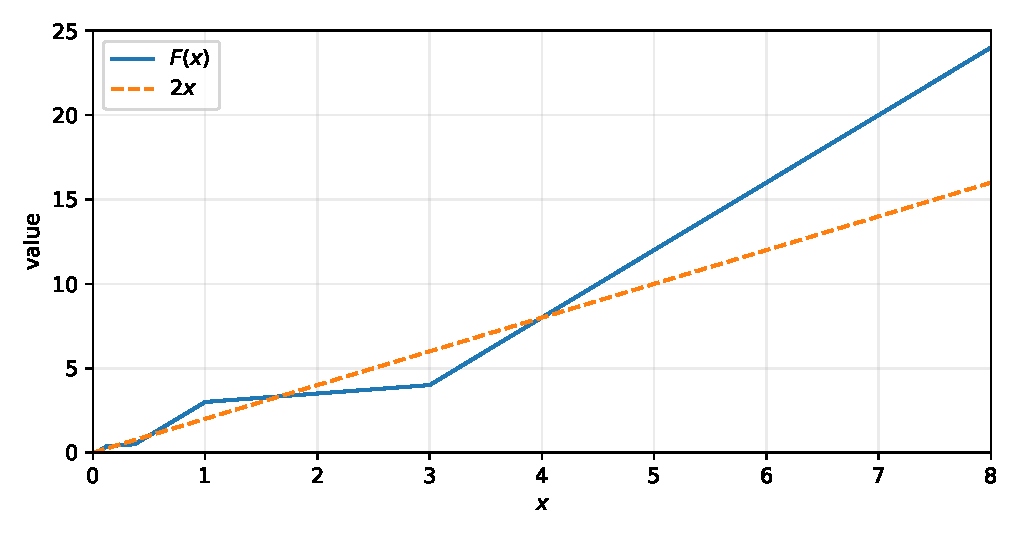
\includegraphics[width=0.88\linewidth]{figures/cubic_counterexample.pdf}
\caption{The exact cubic counterexample on one scale interval, compared
with the homogeneous linear solution. There are infinitely many scaled
copies of the two affine branches, accumulating at zero.}
\label{fig:cubic}
\end{figure}

\subsection{The conjugacy behind the formula}

The construction can also be understood without the itinerary table.
On $[1,8]$ define
\begin{equation}
 h_0(u)=
 \begin{cases}
  2u-1,&1\le u\le2,\\
  u/2+2,&2\le u\le4,\\
  u,&4\le u\le8.
 \end{cases}
 \label{eq:polyH}
\end{equation}
Extend it by $H(8^ku)=8^kh_0(u)$ for $u\in[1,8]$, then extend oddly and set
$H(0)=0$. The map $H$ is an increasing homeomorphism, and it commutes with
$D_8(x)=8x$. Direct calculation shows
\begin{equation}
  F=H\circ D_2\circ H^{-1}.
  \label{eq:conjF}
\end{equation}
Consequently,
\begin{equation}
 \itn{F}{3}=H\circ D_8\circ H^{-1}=D_8.
\end{equation}
The middle equality is useful only because $H$ commutes with $D_8$;
it need not commute with $D_2$.

There is a general warning here. Arbitrary nonlinear conjugacy does
\emph{not} preserve an arbitrary linear combination of iterates.
Although iterates conjugate one by one, a nonlinear conjugating map cannot
be moved through a sum. In \eqref{eq:conjF}, commutation with the specific
third iterate supplies the extra fact needed. In later constructions,
we impose a linear difference equation on the conjugating coordinate
itself instead.

\subsection{A visible failure of differentiability}

The scaled sequences $x_n=8^{-n}$ and $y_n=3\cdot8^{-n}$ both tend to zero,
but
\begin{equation}
  \frac{F(x_n)}{x_n}=3,\qquad
  \frac{F(y_n)}{y_n}=\frac43.
\end{equation}
Thus $F$ is not differentiable at zero, despite being globally
bi-Lipschitz. Section~\ref{sec:regularity} explains why this is inevitable
for a square-free circular spectrum of radius different from $1$.
The next example avoids this regularity issue altogether.

\section{A real-analytic counterexample on the entire real line}
\label{sec:analytic}

Let
\begin{equation}
  h(t)=t+\frac14\sin\frac{\pi t}{2},\qquad
  f(x)=h\bigl(h^{-1}(x)+1\bigr).
  \label{eq:analytic}
\end{equation}
Here $h^{-1}$ is the ordinary inverse function, not a reciprocal.
Since
\begin{equation}
  h'(t)=1+\frac\pi8\cos\frac{\pi t}{2}
  \quad\text{and}\quad
  1-\frac\pi8>0,
\end{equation}
$h$ is strictly increasing. Also $|h(t)-t|\le1/4$, so it maps $\R$ onto
$\R$. Its derivative never vanishes. The real-analytic inverse function
theorem, applied at each real point, makes $h^{-1}$ and $f$ real analytic.
No global complex-analytic inverse is asserted or required.

\begin{theorem}[Analytic quartic counterexample]
\label{thm:quartic}
The function in \eqref{eq:analytic} is an increasing, globally bi-Lipschitz,
real-analytic homeomorphism of $\R$. Its minimal iterative polynomial is
\begin{equation}
  \mu_f(z)=(z-1)^2(z^2+1)
   =z^4-2z^3+2z^2-2z+1.
  \label{eq:quarticP}
\end{equation}
It also satisfies $\itn{f}{4}(x)=x+4$. The equation obtained by deleting the
nonreal roots from \eqref{eq:quarticP} is not satisfied.
\end{theorem}

\begin{proof}
Conjugacy gives, for every integer $n$,
\begin{equation}
  \itn{f}{n}(h(t))=h(t+n)
  =t+n+\frac14\sin\frac{\pi(t+n)}2.
  \label{eq:analyticorbit}
\end{equation}
The linear polynomial in $n$ is killed by $(E-1)^2$, where $E$ shifts
$n$ to $n+1$. The sine term is killed by $E^2+1$. The two operators
commute, so their product kills the entire sequence. Therefore
$\mu_f[f]=0$. Periodicity of the sine also gives $h(t+4)=h(t)+4$, proving
$\itn{f}{4}(x)=x+4$.

The first orbit values at zero are
\begin{equation}
  0,\quad\frac54,\quad2,\quad\frac{11}4,\quad4,
  \quad\frac{21}4,\quad6,\ldots.
  \label{eq:analyticvalues}
\end{equation}
Their $4\times4$ Hankel determinant is
\begin{equation}
 \det\begin{pmatrix}
  0&5/4&2&11/4\\
  5/4&2&11/4&4\\
  2&11/4&4&21/4\\
  11/4&4&21/4&6
 \end{pmatrix}=1.
 \label{eq:quarticdet}
\end{equation}
The same argument used for \eqref{eq:hankelF} rules out every relation of
degree below four. This proves minimality.

After deleting $i$ and $-i$, the remaining polynomial is $(z-1)^2$.
At $x=0$ its residual is
\begin{equation}
 \itn{f}{2}(0)-2f(0)+0=2-2\cdot\frac54=-\frac12.
 \label{eq:analyticresidual}
\end{equation}
Thus the proposed deletion fails. Finally,
$f'(h(t))=h'(t+1)/h'(t)$ is bounded above and bounded away from zero,
which proves the bi-Lipschitz assertion.
\end{proof}

All roots in \eqref{eq:quarticP} lie on the unit circle, and $1$ is a real
root of maximal modulus. This gives a second negative answer, now with
real analyticity at every real point and with all polynomial coefficients
nonzero. Notice that the map has no fixed point: $h(t+1)>h(t)$.
The distinction between a fixed point and a translation-like orbit will
account for the different multiplicity rules at radius $1$.

\begin{figure}[htbp]
\centering
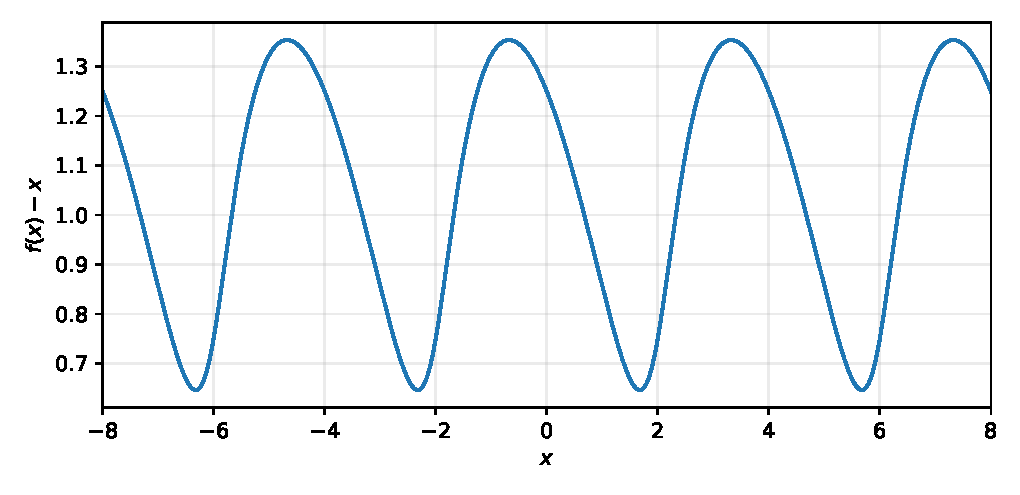
\includegraphics[width=0.88\linewidth]{figures/analytic_displacement.pdf}
\caption{Numerical illustration of $f(x)-x$ for \eqref{eq:analytic}.
The displacement is nonconstant and $4$-periodic. The identities and the
counterexample are established exactly in the text, not by this plot.}
\label{fig:analytic}
\end{figure}

\section{Orbit recurrences and minimal iterative polynomials}
\label{sec:orbits}

We now develop the tools for a general classification. The results in this
section also explain why an exact orbit determinant is a valid
minimality certificate.

\subsection{The annihilator ideal}

\begin{definition}
For a function $f:\R\to\R$, let
\begin{equation}
  \Ann(f)=\{P\in\R[z]:P[f](x)=0\text{ for every }x\in\R\}.
\end{equation}
If this set contains a nonzero polynomial, its monic polynomial of least
degree is called the \emph{minimal iterative polynomial} and is denoted
by $\mu_f$.
\end{definition}

\begin{lemma}
\label{lem:ideal}
The set $\Ann(f)$ is an ideal of $\R[z]$. When it is nonzero,
$\Ann(f)=(\mu_f)$.
\end{lemma}

\begin{proof}
Closure under addition and scalar multiplication is immediate. For every
polynomial $P$,
\begin{equation}
  (zP)[f](x)=P[f](f(x)).
  \label{eq:rightcomp}
\end{equation}
Thus $P\in\Ann(f)$ implies $zP\in\Ann(f)$, and consequently every
polynomial multiple of $P$ belongs to the ideal. Divide any annihilator
by the monic least-degree one. The remainder is another annihilator and
has smaller degree, so it must be zero.
\end{proof}

It is \emph{right composition} in \eqref{eq:rightcomp} that respects
linear combinations. Applying $f$ to a linear combination of its iterates
would not give the same conclusion.

\subsection{Why both forward and backward iterates exist}

\begin{lemma}
\label{lem:homeo}
If $f:\R\to\R$ is continuous and $P[f]=0$ for a polynomial with
$P(0)\ne0$, then $f$ is a strictly monotone homeomorphism of $\R$.
\end{lemma}

\begin{proof}
If $f(x)=f(y)$, then every positive iterate has the same value at $x$ and
$y$. Subtracting the two equations $P[f](x)=P[f](y)=0$ gives
$P(0)(x-y)=0$, hence $x=y$. A continuous injective real function is
strictly monotone.

If its image were a proper interval, at least one of its limits at
$+\infty$ and $-\infty$ would be finite. Along the corresponding end,
$f(x)$ would tend to a finite number, and continuity would make every
positive iterate tend to a finite number as well. But the term $P(0)x$
in the equation would be unbounded. This contradiction proves
surjectivity. A continuous strictly monotone bijection of $\R$ has a
continuous inverse.
\end{proof}

For such an $f$, define $\itn{f}{n}$ for every $n\in\Z$ using inverse
iterates when $n<0$. For any starting point $x$, its orbit
$u_x(n)=\itn{f}{n}(x)$ satisfies
\begin{equation}
  \sum_{j=0}^d a_j u_x(n+j)=0\qquad(n\in\Z).
  \label{eq:recurrence}
\end{equation}
Indeed, substitute $\itn{f}{n}(x)$ into $P[f]=0$.

\subsection{Exponential-polynomial solutions}

\begin{lemma}[Two-sided recurrence decomposition]
\label{lem:recurrence}
Let $P$ be a polynomial with nonzero leading and constant coefficients.
Write its distinct complex roots as $\lambda$, with multiplicities
$m_\lambda$. Every complex sequence $u:\Z\to\C$ satisfying
$P(E)u=0$ has a unique representation
\begin{equation}
  u(n)=\sum_\lambda p_\lambda(n)\lambda^n,
  \qquad \degree p_\lambda<m_\lambda.
  \label{eq:expoly}
\end{equation}
For a real sequence, conjugate roots have conjugate coefficient
polynomials. Its minimal recurrence polynomial is
\begin{equation}
  \prod_{p_\lambda\ne0}
     (z-\lambda)^{1+\degree p_\lambda}.
  \label{eq:minrec}
\end{equation}
\end{lemma}

\begin{proof}
For a polynomial $p$,
\begin{equation}
 (E-\mu)\bigl(p(n)\lambda^n\bigr)
  =\lambda^n\bigl(\lambda p(n+1)-\mu p(n)\bigr).
 \label{eq:shiftdegree}
\end{equation}
When $\mu=\lambda$, a nonconstant polynomial degree drops by one, and a
constant is killed. When $\mu\ne\lambda$, the degree is preserved and the
leading coefficient is multiplied by $\lambda-\mu$.

These observations prove that the proposed sequences satisfy the
recurrence. They also prove their linear independence: in any putative
linear relation, apply enough factors corresponding to all roots except
one. The surviving root component is a nonzero polynomial times an
exponential unless its coefficient polynomial was zero. There are
$\degree P$ independent sequences. A two-sided recurrence with nonzero
first and last coefficients is determined by $\degree P$ consecutive
values, so these sequences form a basis. Formula \eqref{eq:shiftdegree}
then proves the exact multiplicities in \eqref{eq:minrec}.
\end{proof}

\begin{lemma}[From individual orbits to the whole function]
\label{lem:lcm}
The minimal iterative polynomial is the least common multiple of the
minimal recurrence polynomials of all scalar orbits $u_x$. In particular,
for each root, its multiplicity in $\mu_f$ is the maximum of the
multiplicities with which it occurs in the scalar orbits.
\end{lemma}

\begin{proof}
Each orbit is annihilated by $\mu_f$, so its minimal recurrence polynomial
divides $\mu_f$. Conversely, any common multiple of all the orbit
polynomials annihilates every orbit at $n=0$, and hence annihilates $f$.
Only finitely many roots and bounded multiplicities are possible, because
they all occur in $\mu_f$. Therefore their least common multiple and each
stated maximum are attained using finitely many orbits.
\end{proof}

This also gives a finite-dimensional interpretation. Right composition
by $f$ acts linearly on the span of $\id,f,\itn{f}{2},\ldots$.
The vector $\id$ is cyclic, and $\mu_f$ is the minimal polynomial on
this cyclic space. The function $f$ itself need not be linear as a map
of real numbers.

\section{The positivity lemma that controls a circular spectrum}
\label{sec:positivity}

A finite exponential polynomial on the unit circle is a sequence
\begin{equation}
  v(n)=\sum_{\zeta\in S}p_\zeta(n)\zeta^n,
  \qquad n\in\Z,
  \label{eq:unitexp}
\end{equation}
where $S$ is a finite set of distinct complex numbers of modulus one.
The sequence is real when the terms respect conjugation.
The root $\zeta=1$ contributes the nonoscillating polynomial part.

\subsection{A recurrence fact for finite trigonometric sequences}

\begin{lemma}
\label{lem:returns}
For any finite set $S$ on the unit circle, there are positive integers
$N_k\to\infty$ such that $\zeta^{N_k}\to1$ simultaneously for every
$\zeta\in S$. Consequently, for a finite trigonometric sequence
$T(n)=\sum_{\zeta\in S}c_\zeta\zeta^n$ and any fixed $\ell\in\Z$,
\begin{equation}
  T(N_k+\ell)\to T(\ell),\qquad
  T(-N_k+\ell)\to T(\ell).
  \label{eq:returns}
\end{equation}
\end{lemma}

\begin{proof}
The vectors $(\zeta^n)_{\zeta\in S}$ lie in a compact finite product of
circles. Choose a convergent subsequence with indices $n_k$ whose
successive gaps tend to infinity. The componentwise quotient of the
vectors at indices $n_{2k}$ and $n_k$ tends to the identity vector.
Set $N_k=n_{2k}-n_k$. The inverse quotients converge to the identity as
well, giving both assertions in \eqref{eq:returns}.
\end{proof}

\begin{lemma}[Nonnegative trigonometric sequences have positive mean]
\label{lem:mean}
Let $T(n)=\sum_{\zeta\in S}c_\zeta\zeta^n$ be real, nonnegative for every
$n\in\Z$, and not identically zero. Then $1\in S$ and $c_1>0$.
\end{lemma}

\begin{proof}
The Ces\`aro mean of $\zeta^n$ over $n=0,\ldots,N-1$ tends to zero for
$\zeta\ne1$, by the finite geometric-sum formula. Thus the mean of $T$
tends to $c_1$, interpreted as zero if $1\notin S$. Distinctness of the
frequencies gives
\begin{equation}
 \lim_{N\to\infty}\frac1N\sum_{n=0}^{N-1}|T(n)|^2
    =\sum_{\zeta\in S}|c_\zeta|^2>0.
\end{equation}
On the other hand, $0\le T(n)\le M$ for some finite $M$, and
$T(n)^2\le MT(n)$. Taking means proves $c_1>0$.
\end{proof}

\subsection{Parity and dominance of the nonoscillating term}

\begin{theorem}[Two-sided positivity]
\label{thm:positive}
Suppose the real sequence \eqref{eq:unitexp} is nonnegative for all
$n\in\Z$ and is not identically zero. Let
$d=\max\{\degree p_\zeta:p_\zeta\ne0\}$. Then $d$ is even.
The polynomial $p_1$ is present, has degree exactly $d$, and has positive
leading coefficient. The analogous statement for a nonpositive sequence
holds after multiplication by $-1$.
\end{theorem}

\begin{proof}
Let $c_\zeta$ be the coefficient of $n^d$ in $p_\zeta$, with zero used
when its degree is lower, and set
\begin{equation}
  T(n)=\sum_{\zeta\in S}c_\zeta\zeta^n.
\end{equation}
The leading trigonometric sequence is not identically zero, by the
independence in Lemma~\ref{lem:recurrence}. Uniformly as $|n|\to\infty$,
\begin{equation}
 v(n)=n^dT(n)+O(|n|^{d-1}),
 \label{eq:leadingT}
\end{equation}
with the evident exact interpretation when $d=0$.

At $+\infty$, nonnegativity gives $\liminf T(n)\ge0$. Use the first
sequence in \eqref{eq:returns} to conclude $T(\ell)\ge0$ for every fixed
integer $\ell$. At $-\infty$, division by $|n|^d$ and the second return
sequence give $(-1)^dT(\ell)\ge0$ for every $\ell$. If $d$ were odd,
$T$ would vanish identically, a contradiction. Thus $d$ is even.
Lemma~\ref{lem:mean} now gives $c_1>0$. Hence $p_1$ has degree $d$ and the
asserted leading sign.
\end{proof}

The use of both time directions is decisive. For a recurrence constrained
only at nonnegative indices, an odd-degree polynomial may remain
positive. A homeomorphism supplies all negative iterates, eliminating
that possibility.

\begin{corollary}[A vanishing unit-circle exponential polynomial]
\label{cor:vanishing}
If an exponential polynomial \eqref{eq:unitexp} tends to zero as
$n\to+\infty$ or as $n\to-\infty$, it is identically zero.
\end{corollary}

\begin{proof}
Choose its largest polynomial degree $d$ and its leading trigonometric
sequence $T$ as in \eqref{eq:leadingT}. The assumed limit implies
$T(n)\to0$ in the chosen direction. The corresponding return sequence
in Lemma~\ref{lem:returns} gives $T(\ell)=0$ for every $\ell$, contrary
to the choice of a nonzero leading degree. Thus a nonzero exponential
polynomial cannot have the stated limit.
\end{proof}

\section{Classification of minimal polynomials on one circle}
\label{sec:classification}

Call a polynomial \emph{circular of radius $r$} if every one of its complex
roots has modulus $r$. Multiplicities are counted in the usual algebraic
sense. A missing root is assigned multiplicity zero.

\begin{theorem}[Circular-spectrum classification]
\label{thm:classification}
Let $Q\in\R[z]$ be nonconstant and monic, and suppose all its roots lie
on $|z|=r$ for some $r>0$. Then $Q$ is the minimal iterative polynomial
of an increasing homeomorphism $f:\R\to\R$ if and only if the following
conditions hold.
\begin{enumerate}[label=\textnormal{(\roman*)},leftmargin=2.2em]
\item If $r\ne1$, the positive real number $r$ is a root of odd
multiplicity $m_r$, and every other root has multiplicity at most $m_r$.
\item If $r=1$, either $Q(z)=z-1$, or $1$ is a root of even multiplicity
$m_1\ge2$ and every other root has multiplicity at most $m_1-1$.
\end{enumerate}
In case \textnormal{(i)}, realizations can be chosen odd, globally
bi-Lipschitz, and real analytic away from zero. In the nonidentity part of
case \textnormal{(ii)}, realizations can be chosen globally bi-Lipschitz
and real analytic at every real point; they have no fixed point.
\end{theorem}

This is a classification of the polynomials that can be \emph{minimal}.
It is not a parametrization of every function realizing any one polynomial.
The minimality qualification is essential: for example, the identity
satisfies $(z-1)^7[\id]=0$, but its minimal polynomial is only $z-1$.

\subsection{Necessity when \texorpdfstring{$r\ne1$}{r is not 1}}

Let $f$ be increasing and let $\mu_f=Q$. By
Lemma~\ref{lem:recurrence}, every orbit has the form
\begin{equation}
  u_x(n)=r^n\sum_{|\zeta|=1}p_{x,\zeta}(n)\zeta^n.
  \label{eq:circularorbit}
\end{equation}
If $r>1$, this tends to zero as $n\to-\infty$; if $r<1$, it tends to zero
as $n\to+\infty$. Passing to this limit in
$f(u_x(n))=u_x(n+1)$ gives $f(0)=0$.
Since $f$ and $f^{-1}$ are increasing and fix zero, every nonzero orbit
keeps the sign of its starting point for all $n\in\Z$.

For $x>0$, divide \eqref{eq:circularorbit} by $r^n>0$ and apply
Theorem~\ref{thm:positive}. Its largest polynomial degree is even and is
attained by the coefficient of $\zeta=1$, corresponding to the
characteristic root $r$. The same conclusion holds for $x<0$ after a sign
change. Thus, in every nonzero scalar orbit, the multiplicity of $r$ is
odd and is at least as large as every other multiplicity.

Now take the maxima over orbits using Lemma~\ref{lem:lcm}. The maximum of
a nonempty finite set of odd multiplicities is odd. Every other global
multiplicity is bounded by that maximum. This proves the necessity of
condition~(i).

\subsection{Necessity on the unit circle}

Suppose $r=1$ and $f\ne\id$. Choose a nonfixed starting point $x$.
Because $f$ is increasing, the difference sequence
\begin{equation}
  v_x(n)=u_x(n+1)-u_x(n)
  \label{eq:increments}
\end{equation}
has a strict, constant sign for all $n\in\Z$.

Taking a first difference lowers the degree of the polynomial component
at the root $1$ by one. At every other root it preserves the degree,
as \eqref{eq:shiftdegree} shows. Apply Theorem~\ref{thm:positive} to
$v_x$, after a sign change if necessary. Its largest degree is even and
is attained at $1$. Therefore the polynomial component of $u_x$ at $1$
has odd degree $d\ge1$, and every oscillatory component has degree at most
$d-1$. Equivalently, this orbit has an even multiplicity $d+1$ at $1$,
strictly larger than all the other multiplicities.

The nonoscillating leading term dominates the orbit at both ends:
\begin{equation}
  u_x(n)=a n^d+O(|n|^{d-1}),\qquad a\ne0,\quad d\text{ odd}.
  \label{eq:unitgrowth}
\end{equation}
In particular, the two time tails go to opposite infinities. If $f$ had
a fixed point, an increasing orbit starting on either side of it could
never cross it, contradicting \eqref{eq:unitgrowth}. Hence a nonidentity
$f$ in this setting has no fixed point, and all its orbits are nonfixed.
Lemma~\ref{lem:lcm} now gives an even maximal multiplicity at $1$ and the
strict bound on every other multiplicity. If instead $f=\id$, the minimal
polynomial is $z-1$. This proves condition~(ii).

\subsection{Encoding the remaining root directions}

For the construction, write every root other than the distinguished
positive root using an angle $0<\theta_j\le\pi$. An angle
$0<\theta_j<\pi$ denotes the conjugate pair
$r e^{i\theta_j},r e^{-i\theta_j}$, with common multiplicity $m_j$.
The angle $\theta_j=\pi$ denotes the single real root $-r$, if present,
with multiplicity $m_j$. Choose distinct angles and set
\begin{equation}
  e_j=m_j-1.
\end{equation}
A term $t^{e_j}\cos(\theta_jt)$ then produces precisely the desired degree
in its sampled orbit. At angle $\pi$, the two exponential expressions
for the cosine coincide on integer samples and give the one real root,
not two roots.

\subsection{Construction for \texorpdfstring{$r\ne1$}{r is not 1}}
\label{sec:construction-nonunit}

Write $m_r=2k+1$ and set $a=\log r\ne0$. Choose $C\ge1$ so large that
\begin{equation}
  \frac{k}{\sqrt C}\le\frac{|a|}{2},
\end{equation}
and define
\begin{equation}
  A(t)=(t^2+C)^k,\qquad
  W(t)=A(t)+\sum_j\varepsilon_j t^{e_j}\cos(\theta_jt),\qquad
  h(t)=r^tW(t),
  \label{eq:nonunitH}
\end{equation}
where every $\varepsilon_j$ is positive and sufficiently small.
The permitted multiplicities give $0\le e_j\le2k$.
An explicit sufficient choice is any collection satisfying
\begin{equation}
  \sum_j\varepsilon_j\bigl(|a|+e_j+\theta_j\bigr)
     \le\frac{|a|}{4}.
  \label{eq:eps-nonunit}
\end{equation}
When there are no other roots, the sum is empty.

Here are the estimates that justify the construction. For
$0\le e\le2k$,
\begin{equation}
  |t|^e\le A(t),\qquad
  e|t|^{e-1}\le eA(t)\quad(e\ge1),\qquad
  \frac{|A'(t)|}{A(t)}\le\frac{k}{\sqrt C}.
  \label{eq:Abounds}
\end{equation}
The first inequalities follow separately on $|t|\le1$ and $|t|\ge1$.
The last one follows by maximizing $2k|t|/(t^2+C)$.
Since \eqref{eq:eps-nonunit} implies $\sum_j\varepsilon_j\le1/4$,
\begin{equation}
  \frac34A(t)\le W(t)\le\frac54A(t).
  \label{eq:Wbounds}
\end{equation}
Also
\begin{equation}
 h'(t)=r^t\bigl(aW(t)+W'(t)\bigr).
\end{equation}
The unperturbed expression $aA+A'$ has the sign of $a$ and absolute value
at least $|a|A/2$. Each perturbing expression
\begin{equation}
 a t^{e_j}\cos(\theta_jt)
   +e_jt^{e_j-1}\cos(\theta_jt)
   -\theta_jt^{e_j}\sin(\theta_jt)
\end{equation}
has absolute value at most $(|a|+e_j+\theta_j)A(t)$, with the middle term
omitted for $e_j=0$. Thus
\begin{equation}
 \sgn h'(t)=\sgn a,\qquad
 \frac{|a|}{4}r^tA(t)\le |h'(t)|\le\frac{7|a|}{4}r^tA(t).
 \label{eq:Hderiv}
\end{equation}

It follows that $h$ is a real-analytic bijection from $\R$ onto
$(0,\infty)$: it is increasing for $r>1$ and decreasing for $r<1$.
Define
\begin{equation}
  f(x)=h\bigl(h^{-1}(x)+1\bigr)\quad(x>0),\qquad
  f(0)=0,\qquad f(-x)=-f(x).
  \label{eq:nonunitf}
\end{equation}
Even when $h$ is decreasing, the composition in \eqref{eq:nonunitf} is
increasing. Its limit at zero is zero, so the odd extension is an
increasing homeomorphism of $\R$.

Every orbit on the positive half-line is $h(t+n)$. Expanding its cosine
terms shows that it is annihilated by $Q$. Oddness handles negative
orbits. More importantly, at the starting point $h(0)$ the sampled
sequence is
\begin{equation}
  h(n)=r^n\left((n^2+C)^k+
         \sum_j\varepsilon_j n^{e_j}\cos(\theta_jn)\right).
  \label{eq:fullorbit}
\end{equation}
The component at $r$ has degree exactly $2k$, and every other component
has exactly its assigned degree $e_j$, with nonzero leading coefficient.
Lemma~\ref{lem:recurrence} proves that this single orbit has minimal
polynomial $Q$. Hence $\mu_f=Q$.

Finally, \eqref{eq:Hderiv} bounds
$f'(h(t))=h'(t+1)/h'(t)$ above and away from zero, because
$A(t+1)/A(t)$ is positive, continuous, and tends to $1$ at both ends.
The resulting derivative bounds extend to secant bounds across zero.
This proves the bi-Lipschitz and regularity assertions in case~(i).

\subsection{Construction on the unit circle}
\label{sec:construction-unit}

For the identity case choose $f=\id$. Otherwise write $m_1=2k+2$ and
put
\begin{equation}
 A(t)=\int_0^t(1+s^2)^k\,ds
  =\sum_{\ell=0}^k\binom{k}{\ell}\frac{t^{2\ell+1}}{2\ell+1}.
 \label{eq:unitA}
\end{equation}
Now $A$ is an odd polynomial of degree $2k+1$ and
$A'(t)=(1+t^2)^k>0$. Since $e_j\le2k$, set
\begin{equation}
  h(t)=A(t)+\sum_j\varepsilon_jt^{e_j}\cos(\theta_jt)
  \label{eq:unitH}
\end{equation}
with all $\varepsilon_j>0$ chosen so that
\begin{equation}
 \sum_j\varepsilon_j(e_j+\theta_j)<\frac12.
 \label{eq:eps-unit}
\end{equation}
The same estimates as in \eqref{eq:Abounds}, now relative to $A'$, imply
\begin{equation}
 \frac12(1+t^2)^k<h'(t)<\frac32(1+t^2)^k.
 \label{eq:unitHderiv}
\end{equation}
The polynomial $A$ has degree one more than every perturbing amplitude,
so $h(t)\to\pm\infty$ as $t\to\pm\infty$. Therefore $h$ is a
real-analytic increasing diffeomorphism of $\R$.

Set $f=h\circ T\circ h^{-1}$, where $T(t)=t+1$.
All its orbits are $h(t+n)$ and are annihilated by $Q$.
The orbit $h(n)$ contains a nonoscillating polynomial of degree $2k+1$
and exactly the prescribed oscillating polynomial degrees $e_j$.
Thus its minimal recurrence polynomial, and hence $\mu_f$, is $Q$.
The derivative ratio from \eqref{eq:unitHderiv} is bounded above and
away from zero, proving global bi-Lipschitz continuity. The conjugacy
also gives $f(x)>x$ everywhere and therefore no fixed point.
This completes the sufficiency proof and the proof of
Theorem~\ref{thm:classification}.

\section{Quantitative square-free realizations}
\label{sec:squarefree}

The simplest part of the classification has a particularly transparent
formula. It shows that survival of nonreal roots is not restricted to
roots of unity or to an isolated cubic.

Fix $r>0$, $r\ne1$, and distinct angles
$0<\theta_j\le\pi$. Choose nonzero real amplitudes $\varepsilon_j$ and put
\begin{equation}
 W(t)=1+\sum_{j=1}^q\varepsilon_j\cos(\theta_jt),\qquad
 h(t)=r^tW(t).
 \label{eq:simpleH}
\end{equation}
Let $a=\log r$ and
\begin{equation}
 B=\sum_{j=1}^q|\varepsilon_j|\sqrt{a^2+\theta_j^2}.
 \label{eq:Bbound}
\end{equation}

\begin{proposition}
\label{prop:squarefree}
If $B<|a|$, then the odd extension of
$f=h\circ T\circ h^{-1}$ from $(0,\infty)$ to $\R$ is an increasing
homeomorphism with minimal polynomial
\begin{equation}
 (z-r)
 \prod_{0<\theta_j<\pi}
      \bigl(z^2-2r\cos\theta_j\,z+r^2\bigr)
 \prod_{\theta_j=\pi}(z+r).
 \label{eq:simpleP}
\end{equation}
It is real analytic away from zero, and its positive derivative on either
open half-line satisfies
\begin{equation}
 r\frac{|a|-B}{|a|+B}
   \le f'(x)\le
 r\frac{|a|+B}{|a|-B}.
 \label{eq:simpleLip}
\end{equation}
These are also valid global lower and upper Lipschitz constants.
\end{proposition}

\begin{proof}
Since $B\ge|a|\sum_j|\varepsilon_j|$, the condition gives $W(t)>0$.
Moreover,
\begin{equation}
 aW(t)+W'(t)
 =a+\sum_j\varepsilon_j\bigl(a\cos(\theta_jt)
                                -\theta_j\sin(\theta_jt)\bigr)
\end{equation}
differs from $a$ by at most $B$. Thus $h'$ has the sign of $a$,
and its absolute value lies between $r^t(|a|-B)$ and
$r^t(|a|+B)$. This proves that $h$ is a suitable coordinate, and taking
the ratio at $t+1$ and $t$ gives \eqref{eq:simpleLip}. Minimality follows
from the nonzero frequency components in $h(n)$, exactly as before.
\end{proof}

For example, taking one angle $0<\theta<\pi$ yields a nonlinear solution
whose minimal polynomial is
\begin{equation}
  (z-r)(z^2-2r\cos\theta\,z+r^2).
  \label{eq:generalcubic}
\end{equation}
The angle can be any such real number, not necessarily a rational
multiple of $\pi$. In particular, $\theta=\pi/2$ and $r=2$ give the
cubic $z^3-2z^2+4z-8$, all of whose coefficients are nonzero.

A small oscillatory component can coexist with strict monotonicity
because the exponential envelope supplies a nonzero derivative margin.
It is incorrect to infer that an orbit must lose every oscillatory mode
merely because the unnormalized orbit is monotone. The cubic orbit
\eqref{eq:orbitF} makes this visible:
\begin{equation}
 \frac{\itn{F}{n}(1)}{2^n}
   =1,\frac32,1,1,\frac32,1,\ldots.
\end{equation}
The normalized values oscillate, while the actual orbit is strictly
increasing.

\section{Sharp rigidity consequences for increasing solutions}
\label{sec:rigidity}

The classification concerns minimal polynomials, but a given equation
need not be minimal. Passing to divisors gives explicit rigidity tests.

\begin{corollary}[Nonunit circle]
\label{cor:nonunitrigidity}
Let $P$ be a nonconstant monic real polynomial whose roots lie on
$|z|=r\ne1$. If $r$ is not a root, there is no increasing continuous
solution of $P[f]=0$ on $\R$. If $r$ is a root, every increasing continuous
solution is $f(x)=rx$ if and only if
\begin{equation}
  P(z)=(z-r)^m\quad\text{with }m\in\{1,2\}.
  \label{eq:nonunitcriterion}
\end{equation}
\end{corollary}

\begin{proof}
Any such continuous solution is a homeomorphism by
Lemma~\ref{lem:homeo}, and its minimal polynomial divides $P$.
Theorem~\ref{thm:classification} requires the positive root $r$.
Under \eqref{eq:nonunitcriterion}, the only permitted odd multiplicity
is one, so $\mu_f=z-r$.

Conversely, if $P$ has any other root, take that real negative root or
that nonreal conjugate pair together with a simple root at $r$.
The square-free construction realizes the resulting divisor of $P$ as
a minimal polynomial of degree at least two; the realization is not
homogeneous linear. If $P$ has no other root but $m\ge3$, the construction
with $\mu_f=(z-r)^3$ supplies a nonlinear solution. Every solution in
this nonunit setting fixes zero, so affine and homogeneous-linear
rigidity coincide.
\end{proof}

\begin{corollary}[Unit circle]
\label{cor:unitrigidity}
Let $P$ be nonconstant, monic, real, and supported on $|z|=1$.
Let $M$ be the multiplicity of $1$ in $P$.
\begin{enumerate}[label=\textnormal{(\roman*)},leftmargin=2.2em]
\item If $M=0$, there is no increasing continuous solution on $\R$.
\item If $M\ge1$, every increasing continuous solution is the identity
if and only if $M=1$.
\item Among equations with an increasing solution, every increasing
continuous solution is affine if and only if either $M=1$, or
$P(z)=(z-1)^M$ with $M=2$ or $M=3$.
\end{enumerate}
\end{corollary}

\begin{proof}
If $M=0$, the classification rules out every minimal divisor.
If $M=1$, the only possible minimal divisor is $z-1$, regardless of the
multiplicities of the other roots. When $M\ge2$, every translation
$x\mapsto x+c$ satisfies the equation, because its minimal polynomial
for $c\ne0$ is $(z-1)^2$. This proves (i) and (ii).

If $P=(z-1)^M$ with $M=2$ or $3$, the only nonidentity minimal divisor
allowed by the classification is $(z-1)^2$. To see directly that its
solutions are translations, write an orbit as
$\itn{f}{n}(x)=x+n(f(x)-x)$. For $x<y$, order preservation for every
$n\in\Z$ gives
\begin{equation}
  (y-x)+n\bigl((f(y)-y)-(f(x)-x)\bigr)>0.
\end{equation}
The coefficient of $n$ must be zero, so $f(x)-x$ is constant.

If $M\ge4$, a nonlinear realization of $(z-1)^4$ is obtained from
$h(t)=t+t^3/3$. If $M\ge2$ and $P$ has another root, adjoining that
negative root or nonreal conjugate pair to $(z-1)^2$ gives an admissible
minimal divisor of degree greater than two. Its realization cannot be
affine. Indeed, an affine increasing map with slope different from one
has that positive slope as a characteristic root, whereas the only
positive root here is one; an affine map of slope one is a translation
and has minimal degree at most two.
\end{proof}

These criteria make the radius-$1$ boundary especially clear. A simple
positive root at $1$ eliminates all other circular modes for increasing
solutions. A double root at $1$ supplies enough linear drift to allow
nonconstant bounded oscillations. The analytic quartic example realizes
exactly that first nonreal possibility.

\section{What additional regularity does and does not restore}
\label{sec:regularity}

\subsection{Differentiability is enough in the square-free nonunit case}

\begin{theorem}
\label{thm:C1simple}
Let $f:\R\to\R$ be increasing and continuous, and suppose its minimal
iterative polynomial is square-free and supported on $|z|=r\ne1$.
If $f$ is differentiable at zero, then $f(x)=rx$ for every $x$.
\end{theorem}

\begin{proof}
We already know that $f(0)=0$. Write $L=f'(0)$. Differentiating the
iterative relation at zero, using the chain rule and the fixed point,
gives $\mu_f(L)=0$. Since an increasing differentiable map has
$L\ge0$, and zero is not a root, the only possible value is $L=r$.

For a fixed starting point, square-freeness gives
$u(n)=r^nT(n)$, where $T$ is a bounded finite trigonometric sequence.
In the time direction in which $u(n)\to0$, differentiability implies
\begin{equation}
  u(n+1)-ru(n)=o(|u(n)|).
\end{equation}
Divide by $r^{n+1}$ and use boundedness of $T$ to obtain
$T(n+1)-T(n)\to0$. This difference is a unit-circle exponential
polynomial, so Corollary~\ref{cor:vanishing} makes it identically zero.
In particular, $u(1)=ru(0)$. Since the starting point was arbitrary,
$f= r\id$.
\end{proof}

\subsection{A positive-order Taylor remainder handles repeated roots}

\begin{theorem}
\label{thm:holder}
Let $f$ be increasing and continuous, with a minimal iterative polynomial
supported on $|z|=r\ne1$, allowing repeated roots. Suppose $f$ is
differentiable at zero and, for some $\alpha>0$,
\begin{equation}
 f(x)=f'(0)x+O(|x|^{1+\alpha})\qquad(x\to0).
 \label{eq:holder}
\end{equation}
Then $f(x)=rx$ on $\R$. In particular, local $C^{1,\alpha}$ regularity
at zero is sufficient.
\end{theorem}

\begin{proof}
As above, $f(0)=0$ and $f'(0)=r$. Each orbit has the form
$u(n)=r^nv(n)$, where $v$ is a unit-circle exponential polynomial and
$|v(n)|=O((1+|n|)^d)$ for some $d$. Apply \eqref{eq:holder} in the time
direction in which $r^n\to0$. It gives
\begin{align}
 v(n+1)-v(n)
 &=\frac{u(n+1)-ru(n)}{r^{n+1}}\\
 &=O\!\left(r^{\alpha n}(1+|n|)^{d(1+\alpha)}\right)\longrightarrow0.
 \label{eq:holderdecay}
\end{align}
The last limit holds both for $r<1,n\to+\infty$ and for
$r>1,n\to-\infty$. By Corollary~\ref{cor:vanishing}, the difference
vanishes identically. Thus $u(1)=ru(0)$ for every starting point.
\end{proof}

\subsection{\texorpdfstring{$C^1$}{C1} alone is not sufficient with repeated roots}

Consider the particularly simple coordinate
\begin{equation}
 h(t)=e^t(t^2+4),\qquad
 h'(t)=e^t\bigl((t+1)^2+3\bigr)>0.
 \label{eq:C1H}
\end{equation}
Use $f=h\circ T\circ h^{-1}$ on $(0,\infty)$ and extend it oddly through
zero. Its minimal iterative polynomial is $(z-e)^3$.
For $x=h(t)$,
\begin{equation}
 \frac{f(x)}x
  =e\frac{(t+1)^2+4}{t^2+4}\longrightarrow e
       \qquad(t\to-\infty).
\end{equation}
Also $f'(h(t))=h'(t+1)/h'(t)\to e$ as $t\to-\infty$.
Thus the extension is $C^1$ at zero and consequently $C^1$ on $\R$.
It is nonlinear, because its minimal polynomial has degree three.

For every $\alpha>0$, however,
\begin{equation}
 \frac{|f(h(t))-eh(t)|}{h(t)^{1+\alpha}}
 =\frac{e|2t+1|e^{-\alpha t}}{(t^2+4)^{1+\alpha}}
 \longrightarrow\infty\qquad(t\to-\infty).
 \label{eq:notHolder}
\end{equation}
So the positive-order remainder hypothesis of
Theorem~\ref{thm:holder} genuinely strengthens bare differentiability.
The analytic quartic of Section~\ref{sec:analytic}, on the other hand,
shows that even real analyticity cannot restore a universal elimination
rule at radius one, where the map need not have any fixed point.

\section{Exact verification and reproducible artifacts}
\label{sec:verification}

\subsection{What the exact program checks}

The script \texttt{code/verify.py} requires only Python~3.9 or later and
its standard library. All algebraic checks use
\texttt{fractions.Fraction}; there is no floating-point arithmetic in
these certificates. It implements the cubic function in two independent
ways: the direct two-branch scaled formula and the polygonal conjugacy
\eqref{eq:conjF}.

The recorded run tested 4,026 distinct rational starting points, including
positive and negative points, multiple scales, and exact breakpoints.
At every point it checked the cubic identity, oddness, scaling, agreement
of the two implementations, and inverse identities. It also checked
4,025 adjacent exact secant slopes against the bounds $1/2$ and $4$.
These finite tests supplement the all-real branch proof; they are not its
logical replacement.

The program separately verifies recurrences on the integer range
$-80\le n\le80$ and computes nonzero exact Hankel determinants for four
sample orbits. The symbolic exponential-polynomial arguments explain why
the recurrences hold for every integer and why the determinants certify
the stated minimal orders.

\begin{table}[htbp]
\centering
\caption{Exact sample certificates. The companion JSON file records the full
matrices and polynomial coefficients.}
\label{tab:certificates}
\begin{tabularx}{\linewidth}{@{}Xcl@{}}
\toprule
Minimal polynomial & Degree & Hankel determinant\\
\midrule
$z^3-8$ & 3 & $-56$\\
$(z-1)^2(z^2+1)$ & 4 & $1$\\
$(z-2)^3$ & 3 & $-512$\\
$(z-2)^5(z+2)^4(z^2+4)^3$ & 15 & nonzero exact integer\\
\bottomrule
\end{tabularx}
\end{table}

For the degree-15 example the sampled coordinate is
\begin{equation}
 h(n)=2^n\left((n^2+64)^2
       +\frac{n^2}{1024}\cos\frac{\pi n}{2}
       +\frac{n^3}{1024}\cos\pi n\right).
 \label{eq:sample15}
\end{equation}
Every sampled trigonometric value is an integer, so the whole sequence is
rational. The real-variable version satisfies the derivative bounds in
Section~\ref{sec:construction-nonunit}. Indeed, $k=2$, $C=64$,
$1/2<\log2<1$, and $\pi<4$ give
\begin{equation}
 \frac{k}{\sqrt C}=\frac14<\frac{\log2}{2},\qquad
 \frac{2\log2+5+3\pi/2}{1024}
   <\frac{13}{1024}<\frac{\log2}{4}.
\end{equation}
Thus this is not merely a recurrence sequence detached from a monotone
function; the construction realizes it as an actual orbit.

\subsection{Numerical illustration, clearly separated}

The optional script \texttt{code/analytic\_demo.py} evaluates
\eqref{eq:analytic} by bisection. Since $|h(t)-t|\le1/4$, the inverse of
$x$ is bracketed by $x-1/4$ and $x+1/4$ before iteration begins.
On 2,001 points in $[-10,10]$, the recorded double-precision run gave a
maximum absolute quartic residual of approximately $7.11\cdot10^{-15}$
and a maximum absolute residual in $\itn{f}{4}(x)=x+4$ of approximately
$1.24\cdot10^{-14}$. These numbers are implementation checks, not error
bounds valid for all inputs and not part of the proof.

The plotting option generates the two vector figures used in this paper.
The exact script does not require a plotting library. The article's
counterexample remains independently checkable using the three-row
itinerary table and the small integer or rational determinants.

\section{Conclusions and the remaining boundary}
\label{sec:conclusion}

The selected root-elimination question has a definite negative answer
under its stated general hypotheses. The self-similar cubic has a real
root and a nonreal pair at the same maximal modulus, yet every one of
those roots is required by a minimal relation. The analytic quartic
shows that this conclusion is not an artifact of a nonsmooth example.

The circular-spectrum classification identifies the mechanism more
precisely. Away from radius one, positivity of the normalized two-sided
orbit requires an even maximal polynomial degree, producing an odd
multiplicity at the positive root. On the unit circle, it is the orbit
\emph{increment} that must have constant sign; taking the increment
lowers the degree at one, producing an even multiplicity there and a
strict multiplicity margin over every oscillating mode. Small
trigonometric perturbations realize all and only the permitted patterns.

Several boundaries remain outside this report. We have not classified
minimal polynomials with roots on several distinct circles. We have not
classified decreasing homeomorphisms, for which consecutive iterates
reverse order. Nor have we handled noninjective equations with zero
constant coefficient or arbitrary proper interval domains. These are
limitations of the proved statements, not qualifications needed by the
two counterexamples on $\R$.

Finally, mathematical verification and historical priority are different
questions. The paper gives complete arguments and exact finite
certificates; it does not supply an independent referee report or an
exhaustive priority search. The broader linearity problem is not declared
solved. What is established here is the failure of the proposed general
nonreal-root deletion and an exact, constructive classification in the
increasing single-circle setting.

\appendix
\section{Source and status audit}
\label{app:sources}

The literature search was performed on 20 September 2026. The primary
sources below were used to identify the question and delimit the claims,
not to replace the proofs in this article.

\paragraph{The target.}
Draga--Morawiec \cite{DM2016}, Problem~6.1, is present in the retrieved
HTML and in the rendered page~13 of arXiv:1503.00570v2. The preprint has
14 pages. Its published bibliographic record is
\emph{Aequationes Mathematicae} 90 (2016), 935--950, with DOI
\texttt{10.1007/s00010-016-0420-4}. The source is about preserving the
solution equation after reducing the characteristic polynomial, rather
than merely preserving the existence of at least one solution.

\paragraph{Subsequent context.}
Draga's note \cite{D2016} gives another order-reduction theorem and
mentions the unrestricted nonreal-root issue in its final remarks.
The later paper \emph{Means of iterates} \cite{DM2018} treats a particular
family of iterative mean equations and uses characteristic-root
analysis. A 2021 paper \cite{TLM2021} studies a class of fourth-order
equations under restrictions on the characteristic roots. These sources
show continuing work on the subject; none of the retrieved material
established priority for the counterexample developed here.

\paragraph{Initial lead.}
Petrov's question \cite{Petrov2016} was the initial candidate. Its displayed
answer count was zero in the retrieved page. An unanswered question page
is not, by itself, proof that no published solution exists elsewhere.

\paragraph{Search limitation.}
The search included the authors' names, polynomial-like iterative
equations, nonreal-root elimination, equal-modulus roots, and the numbered
problem. Some returned results were irrelevant and were not used. The
search was not a complete citation-database survey. Thus the report does
not attach a first-discovery claim to the elementary construction or to
the classification theorem. The complete source identifiers and this
status distinction are also recorded in
\texttt{notes/literature\_audit.md}.

\section{Reproduction, selection, and exclusion record}
\label{app:reproduce}

From the archive's top-level directory, the following commands reproduce
the exact certificates and, with the optional plotting dependency, the
numerical illustrations:
\begin{lstlisting}
python code/verify.py
python code/analytic_demo.py --plots
pdflatex -interaction=nonstopmode -halt-on-error article.tex
pdflatex -interaction=nonstopmode -halt-on-error article.tex
pdflatex -interaction=nonstopmode -halt-on-error article.tex
\end{lstlisting}
The supplied figure files allow the PDF to be compiled without running
the plotting script. No bibliography processor is required.

The exact verifier normalizes positive rational numbers by multiplication
or division by eight, not by taking an approximate logarithm. This avoids
wrong branch choices at powers of eight. Its independent conjugacy
implementation also uses rational operations. The recurrence polynomials
in the JSON certificate are stored with coefficients in \emph{ascending}
order, so, for example, $z^3-8$ is represented by
\texttt{[-8, 0, 0, 1]}.

The random area draw was:
\begin{center}
\begin{tabular}{ll}
\toprule
Number of listed areas & 80\\
Generator call & \texttt{secrets.randbelow(80)}\\
Returned zero-based index & 17\\
Selected one-based index & 18\\
Selected area & Functional equations\\
Redraws & 0\\
\bottomrule
\end{tabular}
\end{center}
An entropy-backed draw is recorded rather than seed-replayed; running a
new draw is not expected to reproduce the same index. The full 80-element
list is in \texttt{data/selection.json}.

The excluded input was the 1,095-line file \texttt{manifest(1).tex}, with
SHA-256 fingerprint
\begin{center}
\small\ttfamily
729fb6e3aef3f30c7c5284c4296681fba72b6d6af68211f178ad0bc3c5d15b41.
\end{center}
The file was reviewed as an exclusion list; this report does not certify
the correctness or priority of its individual mathematical claims.
A suggested new manifest entry is supplied separately so that future
selections can exclude the present target as well.

\clearpage
\begin{thebibliography}{9}

\bibitem{DM2016}
S.~Draga and J.~Morawiec,
\emph{Reducing the polynomial-like iterative equations order and a
generalized Zolt\'an Boros' problem},
Aequationes Mathematicae \textbf{90} (2016), 935--950.
\href{https://doi.org/10.1007/s00010-016-0420-4}{doi:10.1007/s00010-016-0420-4}.
Preprint: \href{https://arxiv.org/abs/1503.00570v2}{arXiv:1503.00570v2},
1 December 2015. Problem~6.1 is on preprint page~13.

\bibitem{D2016}
S.~Draga,
\emph{A note on the order of polynomial-like iterative equations},
Commentationes Mathematicae \textbf{56} (2016), 243--249.
Preprint title: \emph{A note on the polynomial-like iterative equations
order}, \href{https://arxiv.org/abs/1604.01287v2}{arXiv:1604.01287v2},
14 November 2016.

\bibitem{Petrov2016}
F.~Petrov,
\emph{Continuous linear recurrent relations},
MathOverflow question 232493, 1 March 2016.
\url{https://mathoverflow.net/questions/232493/continuous-linear-recurrent-relations}.
Retrieved 20 September 2026.

\bibitem{DM2018}
S.~Draga and J.~Morawiec,
\emph{Means of iterates},
\href{https://arxiv.org/abs/1801.05006v2}{arXiv:1801.05006v2},
19 February 2018.

\bibitem{TLM2021}
S.~Thangroongvongthana, V.~Laohakosol, and S.~Mavecha,
\emph{A class of continuous solutions of a fourth order polynomial-like
iterative equation},
Current Applied Science and Technology \textbf{21}(3) (2021), 495--523.
\url{https://li01.tci-thaijo.org/index.php/cast/article/view/248735}.

\end{thebibliography}
\end{document}
